% Niveau :      PCSI
% Discipline :  Elec
% Mots clés :   Elec, Ordre 2

\begin{exercise}{Décrement logarithmique}{2}{Sup}{\'Electrocinétique, Circuits d'ordre 2}{correge}

Dans le montage ci-dessous, le générateur de tension est idéal, de force électromotrice $E$ constante. Tant que l'interrupteur est ouvert, le condensateur est déchargé et la bobine (idéale) n'est parcourue par aucun courant. À l'instant $t=0$, on ferme l'interrupteur.

\begin{figure}[H]
\centering
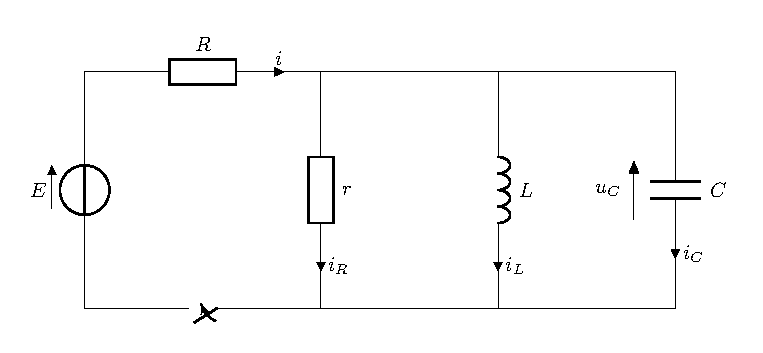
\includegraphics[scale=1]{elec/circuitDecrement.pdf}
\end{figure}

\begin{questions}
    \question Déterminer par raisonnements simples la tension $u$ et les courants $i_R, i_L,i_C$ et $i$ (dans l'ordre qui vous paraîtra le plus judicieux):  à $t=0^-$, à $t=0^+$ et à $t\to \infty$.
    
    \question Établir l'équation différentielle régissant l'évolution de $i_R$ (on pourra écrire la loi des noeuds et la dériver). On posera pour ce circuit parallèle :
              \[\omega_0 = \frac{1}{\sqrt{LC}} \qquad \lambda = \frac{R+r}{2rRC}\]
    \question Pour la suite, on prendra $R=\SI{2,50}{k\ohm}, r=\SI{1,25}{k\ohm}, C=\SI{1,00}{\micro\farad}, L=\SI{20,0}{mH}, E=\SI{6,00}{V}$. À quel type de régime transitoire assiste-t-on ? Justifier.
    \question Définir et calculer la pseudo-pulsation $\omega$ et la pseudo-période $T$ du phénomène. Compte-tenu de la précision des données, que peut-on dire des valeurs numériques comparées de $\omega$ et $\omega_0$ ?
    \question Écrire la solution de l'équation différentielle en $i_R$ obtenue à la question 2 et satisfaisant aux conditions initiales trouvées à la question 1.
    \question En déduire alors l'expression de $u(t)$ et tracer l'allure du graphe correspondant. Donner l'instant $t_0$ auquel $u$ atteint sa valeur maximale.
    \question On définit le décrément logarithmique de $u$ par 
              \[\delta = \frac{1}{n}\ln\left(\frac{u(t)}{u(t+nT)}\right)\]
              Exprimer $\delta$ en fonction de $\lambda$ et $T$. Application numérique.
\end{questions}
\end{exercise}